\chapter{Decoder-Only Transformers: From Blocks to GPT}
\label{ch:decoder-only}

\section{Why Decoder-Only?}

In 2017, the Transformer had two halves: an encoder that reads, and a decoder that writes. By 2020, the most capable language models had thrown away the encoder entirely---no bidirectional attention, no cross-attention, no paired training data. GPT-2 generated coherent paragraphs of text using nothing but the decoder half. GPT-3, a hundred times larger, could answer questions, write code, and translate between languages, all from the same decoder-only architecture trained on a single objective: predict the next token.

Half the original design was discarded, and the remaining half turned out to be more general than the whole. Why?

The answer lies in what language modeling actually asks for. An encoder--decoder assumes a separation between input and output---French goes in, English comes out. But a language model has no separate ``source.'' The input \emph{is} the beginning of the output. When you prompt GPT with a question, the question is not encoded into a separate representation; it becomes the prefix that the model continues. A single stack of causal Transformer blocks handles everything: it reads the prefix through masked self-attention and predicts the next token from the top of the stack.

Three properties made decoder-only the default:

\begin{enumerate}[nosep]
  \item \textbf{One objective, any task.} Next-token prediction on raw text. No paired corpora, no task-specific heads, no encoder warmup. Summarization, translation, code generation, and question answering all reduce to ``continue this prefix.''
  \item \textbf{Data efficiency.} Every token in every document provides a training signal. Classical encoder--decoder translation relies on paired source--target examples; a decoder-only model learns from raw text at scale.
  \item \textbf{Concentrated capacity.} All parameters live in one causal stack. An encoder--decoder splits capacity between two stacks with separate attention pathways---and the decoder must maintain cross-attention to encoder outputs throughout generation, adding complexity without adding generality.
\end{enumerate}

\begin{figure}[t]
  \centering
  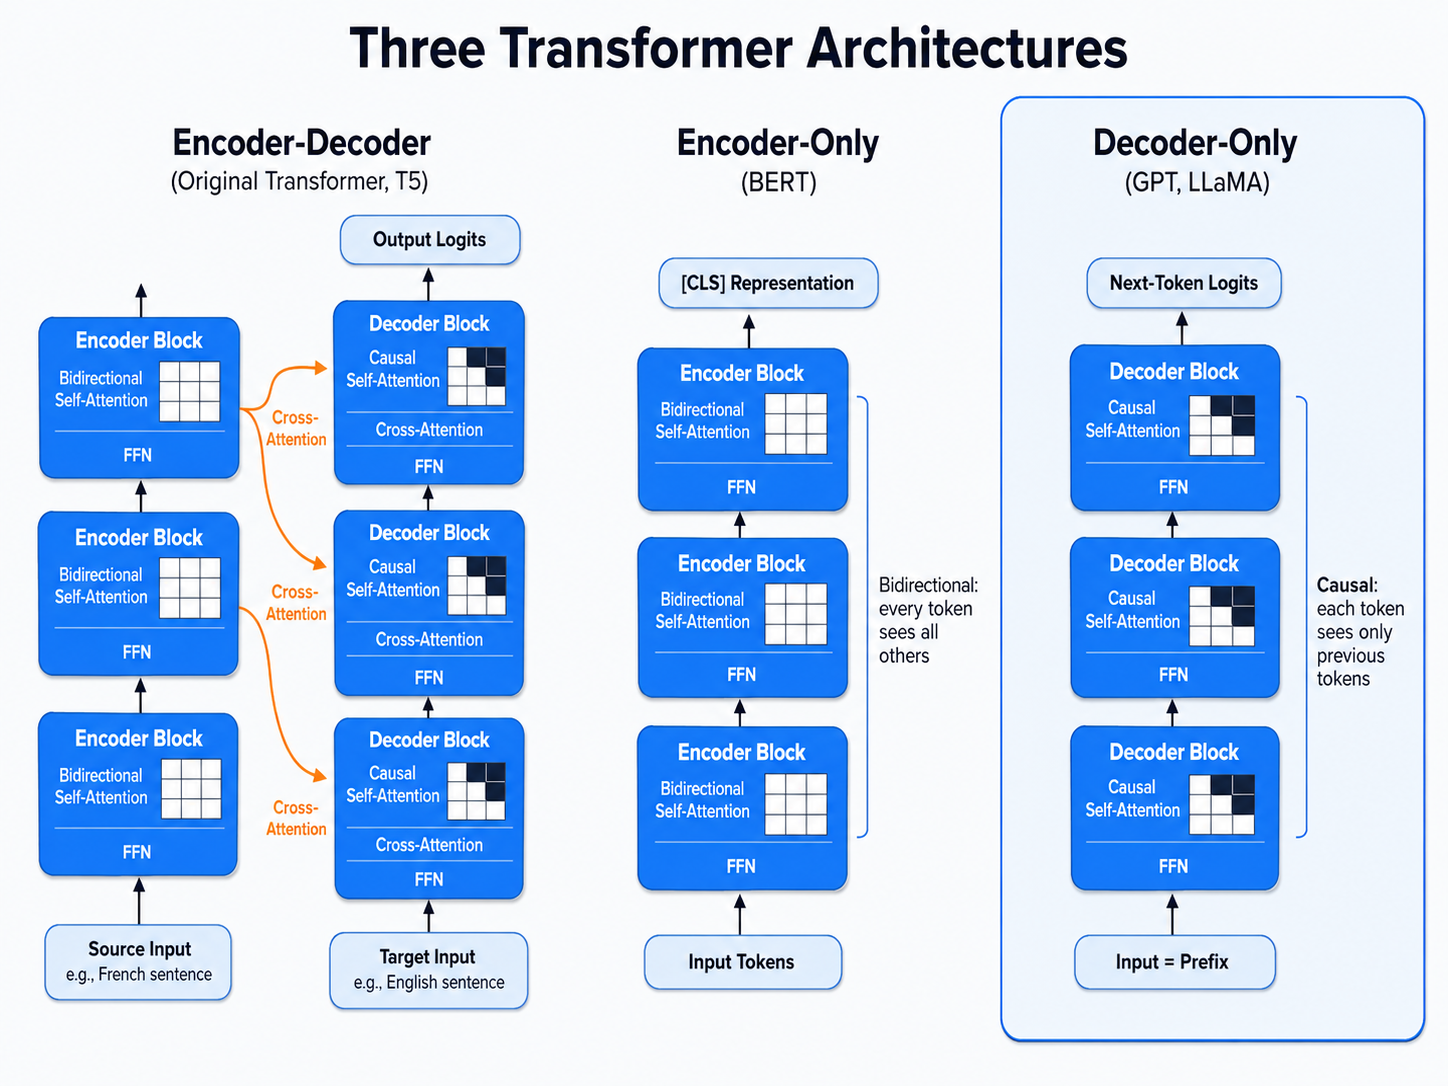
\includegraphics[width=0.9\textwidth]{figures/ch03/three_architectures.png}
  \caption{Three Transformer architecture families, all built from the same attention block (Chapter~\ref{ch:attention}). \textbf{Left:} encoder--decoder, with separate stacks and cross-attention---designed for paired input/output tasks like translation. \textbf{Center:} encoder-only (BERT), with bidirectional attention---designed for representation learning. \textbf{Right:} decoder-only (GPT), with causal masked self-attention---the LLM default. The decoder-only design uses a single stack for both ``understanding'' and generation.}
  \label{fig:three-architectures}
\end{figure}

For comparison, BERT~\cite{devlin2019bert} used only the encoder half---bidirectional attention with a masked language modeling objective. BERT excels at representation and classification tasks but cannot natively generate text: it was trained to fill in blanks, not to extend a prefix. We cover encoder-only architectures in Chapter~\ref{ch:bert}.

\begin{quickrecap}
\textbf{Quick Recap.}
\begin{itemize}[nosep,leftmargin=1.5em]
  \item Encoder--decoder assumes paired input/output; decoder-only treats the input as a prefix to continue.
  \item Next-token prediction on raw text is a universal training objective---no paired data needed.
  \item Decoder-only became the LLM default because of objective simplicity, task unification, and parameter efficiency.
\end{itemize}
\textit{But: saying ``use a decoder'' does not yet specify a model. What does the full forward pass look like?}
\end{quickrecap}


\subsection*{Learning Objectives}

After completing this chapter, you should be able to:

\begin{enumerate}
  \item Trace the full forward pass of a decoder-only Transformer: token ids $\to$ embeddings $\to$ decoder blocks $\to$ logits $\to$ shifted cross-entropy loss.
  \item Explain why the residual stream is the central information highway and how attention/FFN modules read from and write to it.
  \item Compare design choices in modern GPTs: RoPE vs.\ learned PE, SwiGLU vs.\ GELU, GQA vs.\ MHA---and articulate the engineering tradeoff behind each.
  \item Describe how KV caching works, why it is necessary for efficient autoregressive inference, and estimate its memory cost.
  \item Estimate the parameter count of a Transformer given its depth, width, and vocabulary size.
\end{enumerate}

\subsection*{Notation}

The following notation is introduced or formalized in this chapter:

\begin{center}
\begin{tabular}{ll}
\toprule
Symbol & Meaning \\
\midrule
$L$ & Number of Transformer layers (depth) \\
$d_{\text{model}}$ & Hidden dimension (width) of the residual stream \\
$d_{\text{ff}}$ & FFN intermediate dimension (typically $4 d_{\text{model}}$ or $\frac{8}{3} d_{\text{model}}$) \\
$V$ & Vocabulary size \\
$T$ & Sequence length (context window) \\
$n_{\text{kv}}$ & Number of key-value heads (GQA); equals $h$ in standard MHA \\
$\mathbf{x}_t$ & Residual-stream vector at position $t$ \\
\bottomrule
\end{tabular}
\end{center}

\subsection*{Timeline}

This chapter traces the evolution from the original Transformer to modern decoder-only LLMs. The pace is striking: six years separated the architecture from its largest deployments, but the core structure barely changed---what changed was scale, components, and engineering discipline.

\begin{center}
\begin{tabularx}{\textwidth}{@{}lp{3.8cm}X@{}}
\toprule
Year & Contribution & Key idea \\
\midrule
2017 & Transformer & Encoder--decoder self-attention; parallel sequence processing \\
2018 & GPT-1 & Decoder-only pretraining + fine-tuning \\
2019 & GPT-2 & Zero-shot transfer from decoder-only LM; pre-norm, learned PE \\
2020 & GPT-3 & 175B parameters; few-shot in-context learning \\
2020 & SwiGLU & Gated FFN activation; fewer dead neurons \\
2021 & RoPE & Rotary position encoding: relative position via Q/K rotation \\
2023 & LLaMA & Open-weight recipe: RoPE + SwiGLU + pre-norm \\
2023 & Mistral/Qwen & GQA becomes common in larger and later open-weight models \\
\bottomrule
\end{tabularx}
\end{center}


%----------------------------------------------------------------------
\section{The GPT Forward Pass}
\label{sec:gpt-forward}

We start with the simplest decoder-only Transformer---essentially GPT-2~\cite{radford2019language}---and trace every step from raw text to training loss. To make this concrete, we will follow a single example through the entire pipeline.

\paragraph{Running example.} Suppose our vocabulary has 50{,}257 tokens (GPT-2's actual vocabulary size), our model has $d_\text{model} = 768$, $L = 12$ layers, and $h = 12$ heads. The input is the string \texttt{"The cat sat on"}, which the tokenizer maps to four token ids: $(464, 3797, 3332, 319)$. Our goal: produce a probability distribution over the next token.

\subsection{Token Embedding and Positional Encoding}

Each token id indexes into an \textbf{embedding table} $\mathbf{E} \in \mathbb{R}^{V \times d_\text{model}}$---a lookup, not a computation. Token 464 pulls out the 464th row of $\mathbf{E}$, producing a 768-dimensional vector. Position information is then added:
\[
  \mathbf{x}_t^{(0)} = \mathbf{E}_{w_t} + \mathbf{PE}_t
\]
where $\mathbf{PE}_t$ is the positional encoding for position $t$ (learned in GPT-2; we discuss modern alternatives in \S\ref{sec:position-modern}). After this step, our running example is a $4 \times 768$ matrix: four vectors, one per token, each carrying both content and position information.

\medskip
\noindent\fbox{\parbox{\dimexpr\textwidth-2\fboxsep-2\fboxrule\relax}{\textbf{Pause and verify.} Why does this step use addition ($\mathbf{E}_{w_t} + \mathbf{PE}_t$) rather than concatenation ($[\mathbf{E}_{w_t}; \mathbf{PE}_t]$)? What would concatenation do to the dimensionality of the residual stream? Think about this before reading on.}}
\medskip

Addition keeps the dimensionality at $d_{\text{model}}$, so every downstream layer---attention, FFN, output head---operates on the same fixed width. Concatenation would double the dimension and break this uniformity. In practice, the model learns to dedicate some dimensions primarily to content and others primarily to position, even though both are summed into the same vector.

\subsection{The Decoder Block Stack}

Our $4 \times 768$ matrix now passes through $L = 12$ identical decoder blocks. Each block applies causal multi-head attention and a feed-forward network, both wrapped in residual connections and layer normalization (Chapter~\ref{ch:attention}):
\[
  \mathbf{z}^{(\ell)} = \mathbf{x}^{(\ell)} + \text{MHA}\!\big(\text{LN}(\mathbf{x}^{(\ell)})\big)
\]
\[
  \mathbf{x}^{(\ell+1)} = \mathbf{z}^{(\ell)} + \text{FFN}\!\big(\text{LN}(\mathbf{z}^{(\ell)})\big)
\]
This is the \emph{pre-norm} formulation: normalize \emph{before} each sub-layer, not after. After the final block, one last LayerNorm is applied:
\[
  \mathbf{h}_t = \text{LN}\!\big(\mathbf{x}_t^{(L)}\big)
\]

\begin{figure}[t]
  \centering
  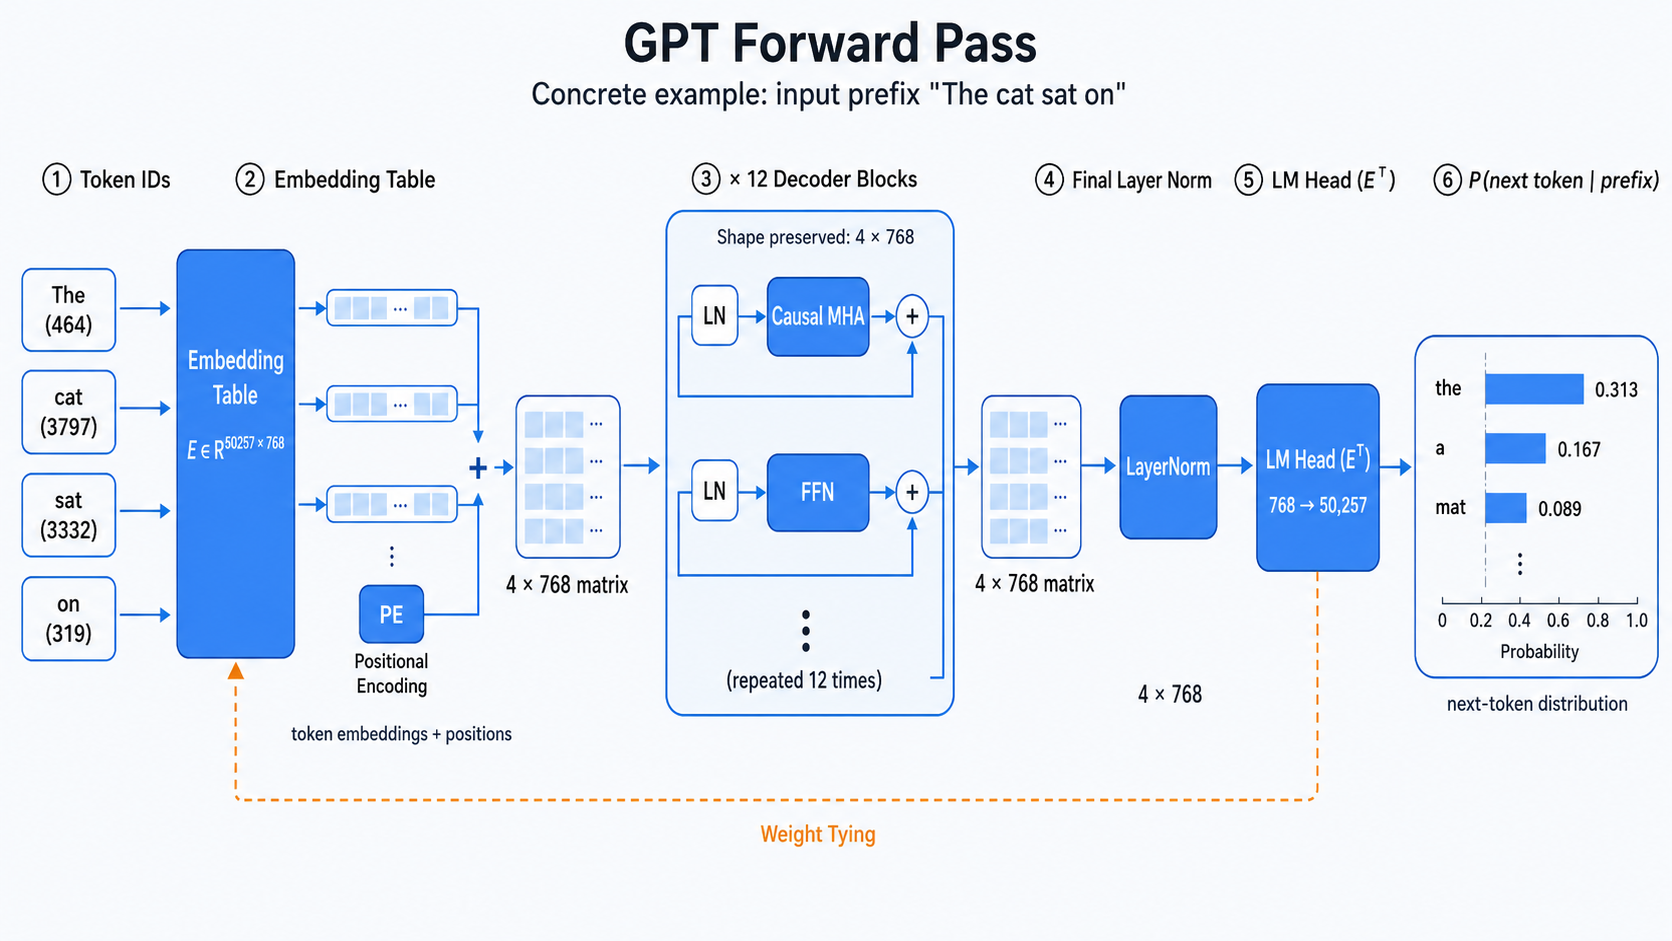
\includegraphics[width=0.85\textwidth]{figures/ch03/gpt_forward_pass.png}
  \caption{The GPT forward pass traced on a running example. Token ids are looked up in the embedding table, combined with positional encoding, passed through $L$ decoder blocks (each applying causal self-attention and an FFN to the residual stream), then projected through the LM head to produce next-token logits. Weight tying shares parameters between the embedding table and the output projection (dashed arrow).}
  \label{fig:gpt-forward}
\end{figure}

In our running example, the matrix stays $4 \times 768$ throughout---the shape never changes, only the content. After 12 blocks of attention-mediated mixing and per-token FFN transformation, each row has been enriched with information from all preceding positions. The vector for ``on'' (position 4) now encodes not just the token itself but the fact that a cat sat on something, and the model is ready to predict what comes next.

\subsection{The Language Modeling Head}

The final hidden state $\mathbf{h}_t$ is projected to a distribution over the entire vocabulary:
\[
  \text{logits}_t = \mathbf{W}_{\text{lm}} \, \mathbf{h}_t \in \mathbb{R}^V
\]
In our running example, the 768-dimensional vector for ``on'' is multiplied by a $50{,}257 \times 768$ matrix, producing 50{,}257 logits---one score per token in the vocabulary. After softmax, this becomes a probability distribution. If training has gone well, tokens like ``the,'' ``a,'' or ``top'' should receive high probability; tokens like ``quantum'' or ``xylophone'' should receive almost zero.

\paragraph{Weight tying.} In GPT-2, LLaMA, and most modern LLMs, the LM head matrix $\mathbf{W}_{\text{lm}}$ is not a separate parameter---it \emph{is} the embedding table transposed: $\mathbf{W}_{\text{lm}} = \mathbf{E}^\top$. This saves $V \times d_{\text{model}}$ parameters (38.6M for GPT-2, hundreds of millions for larger models) and enforces a satisfying symmetry: the same vector that represents a token as input also defines what ``closeness to that token'' means in the output. Tokens with similar embeddings will compete with each other in the softmax.

\subsection{Shifted Cross-Entropy Loss}

The training signal is deceptively simple: at every position, predict the next token. Labels are just the input shifted by one:
\begin{align*}
  \text{input:} \quad & \texttt{The}, \; \texttt{cat}, \; \texttt{sat}, \; \texttt{on} \\
  \text{target:} \quad & \texttt{cat}, \; \texttt{sat}, \; \texttt{on}, \; \texttt{the}
\end{align*}
\begin{figure}[t]
  \centering
  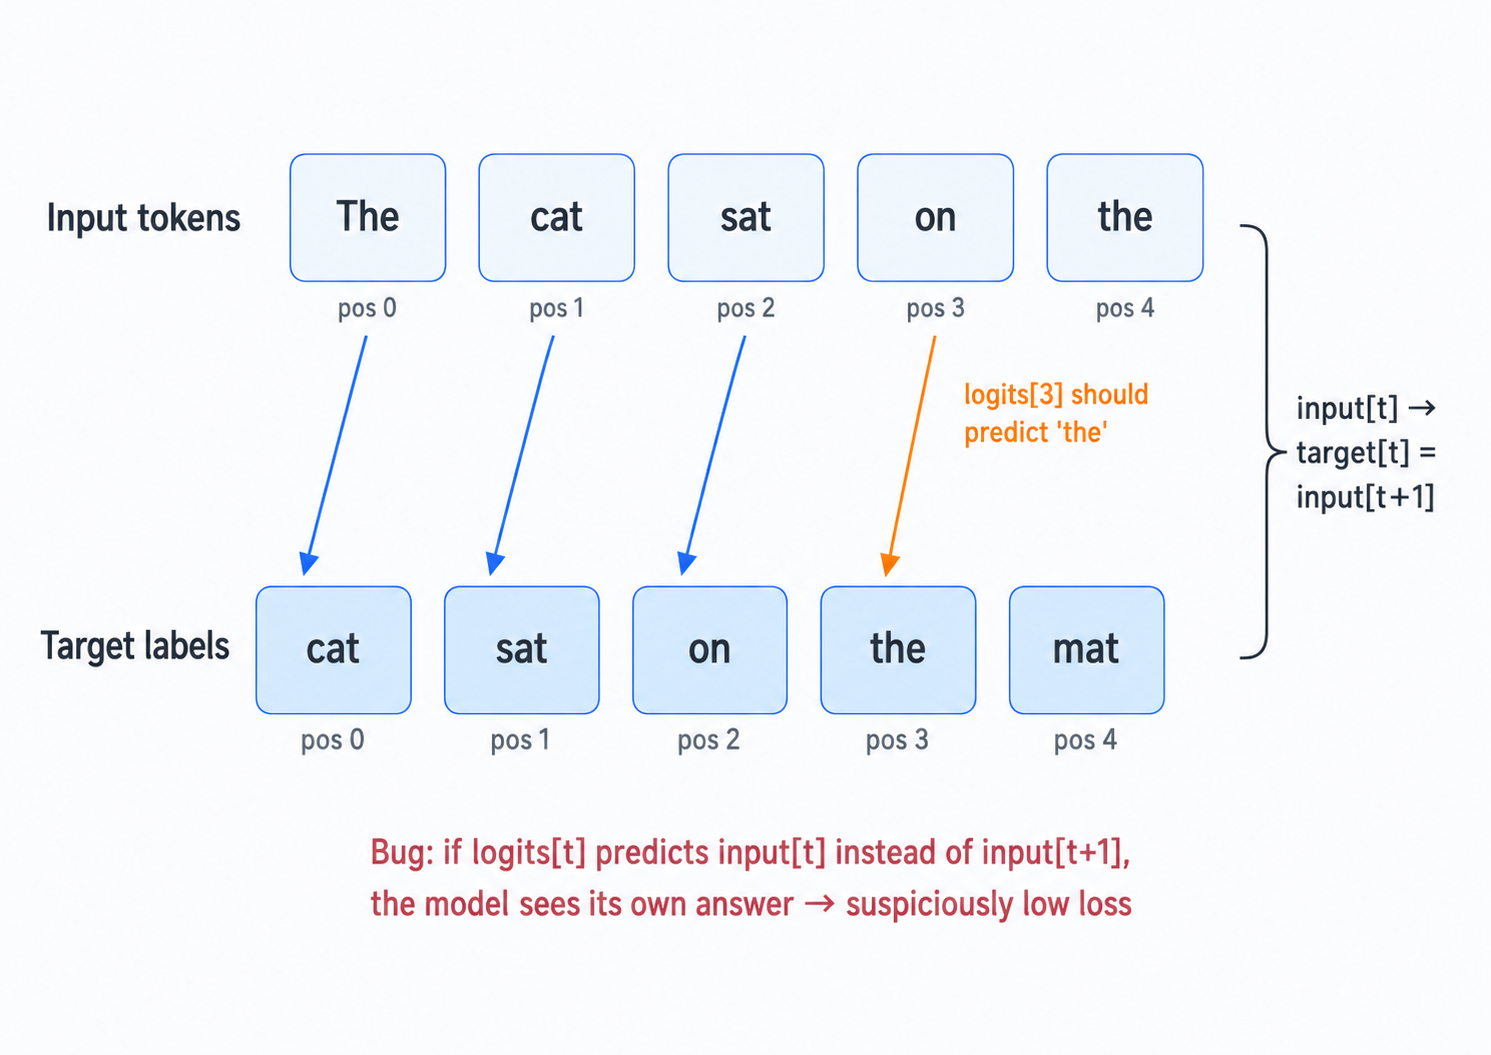
\includegraphics[width=0.85\textwidth]{figures/ch03/shifted_labels.png}
  \caption{Next-token prediction training: logits at position $t$ are supervised by the token at position $t+1$. The input and target sequences are the same text shifted by one position. Misaligning this shift---so that logits predict the \emph{current} token instead of the next---is a common silent bug that produces misleadingly low loss.}
  \label{fig:shifted-labels}
\end{figure}

The loss is cross-entropy averaged over all positions:
\[
  \mathcal{L} = -\frac{1}{T-1} \sum_{t=1}^{T-1} \log P_\theta(w_{t+1} \mid w_{\leq t})
\]
Every token in every document provides one training example. A 300-billion-token corpus yields 300 billion gradient signals---no labeling, no pairing, no curation. This is the engine behind large-scale pretraining.

\paragraph{The off-by-one bug.} If the logits and labels are not correctly shifted, the model trains on trivially easy targets (predicting the current token instead of the next) or silently skips the first position. The training loss will look fine---suspiciously fine. Always verify alignment: \texttt{logits[:, :-1]} should match \texttt{labels[:, 1:]}. This is the GPT equivalent of the mask bug from Chapter~\ref{ch:attention}: a silent failure that produces misleadingly good numbers.

\begin{quickrecap}
\textbf{Quick Recap.}
\begin{itemize}[nosep,leftmargin=1.5em]
  \item Full forward pass: token ids $\to$ embedding + PE $\to$ $L$ decoder blocks $\to$ final LN $\to$ LM head $\to$ logits.
  \item Weight tying shares parameters between the embedding table and the output projection, saving $V \times d_\text{model}$ parameters.
  \item Training loss is cross-entropy on shifted labels: logits at position $t$ are supervised by the token at position $t+1$.
  \item Off-by-one label alignment is a common silent bug---always verify the shift.
\end{itemize}
\textit{So far the decoder block is a black box. What is actually happening inside---and why does stacking 32, 64, or 128 of them work at all?}
\end{quickrecap}


%----------------------------------------------------------------------
\section{The Residual Stream}
\label{sec:residual-stream}

Ask someone to draw a Transformer and they will draw a stack of attention layers. This is wrong---or at least, it puts the emphasis in the wrong place. The primary data structure in a decoder-only Transformer is not attention. It is the \textbf{residual stream}: a $T \times d_{\text{model}}$ matrix that flows from the embedding table all the way to the output head, modified only by additive contributions from attention and FFN sub-layers along the way.

Think of a river with tributaries. The river (the residual stream) flows continuously from source to mouth. Attention and FFN blocks are tributaries that contribute new information---but the river is never dammed and rebuilt. Each decoder block adds to the stream; it does not replace it:
\[
  \mathbf{x}^{(\ell+1)}_t = \mathbf{x}^{(\ell)}_t + \underbrace{\text{MHA output}}_{\text{inter-token}} + \underbrace{\text{FFN output}}_{\text{intra-token}}
\]

\begin{figure}[t]
  \centering
  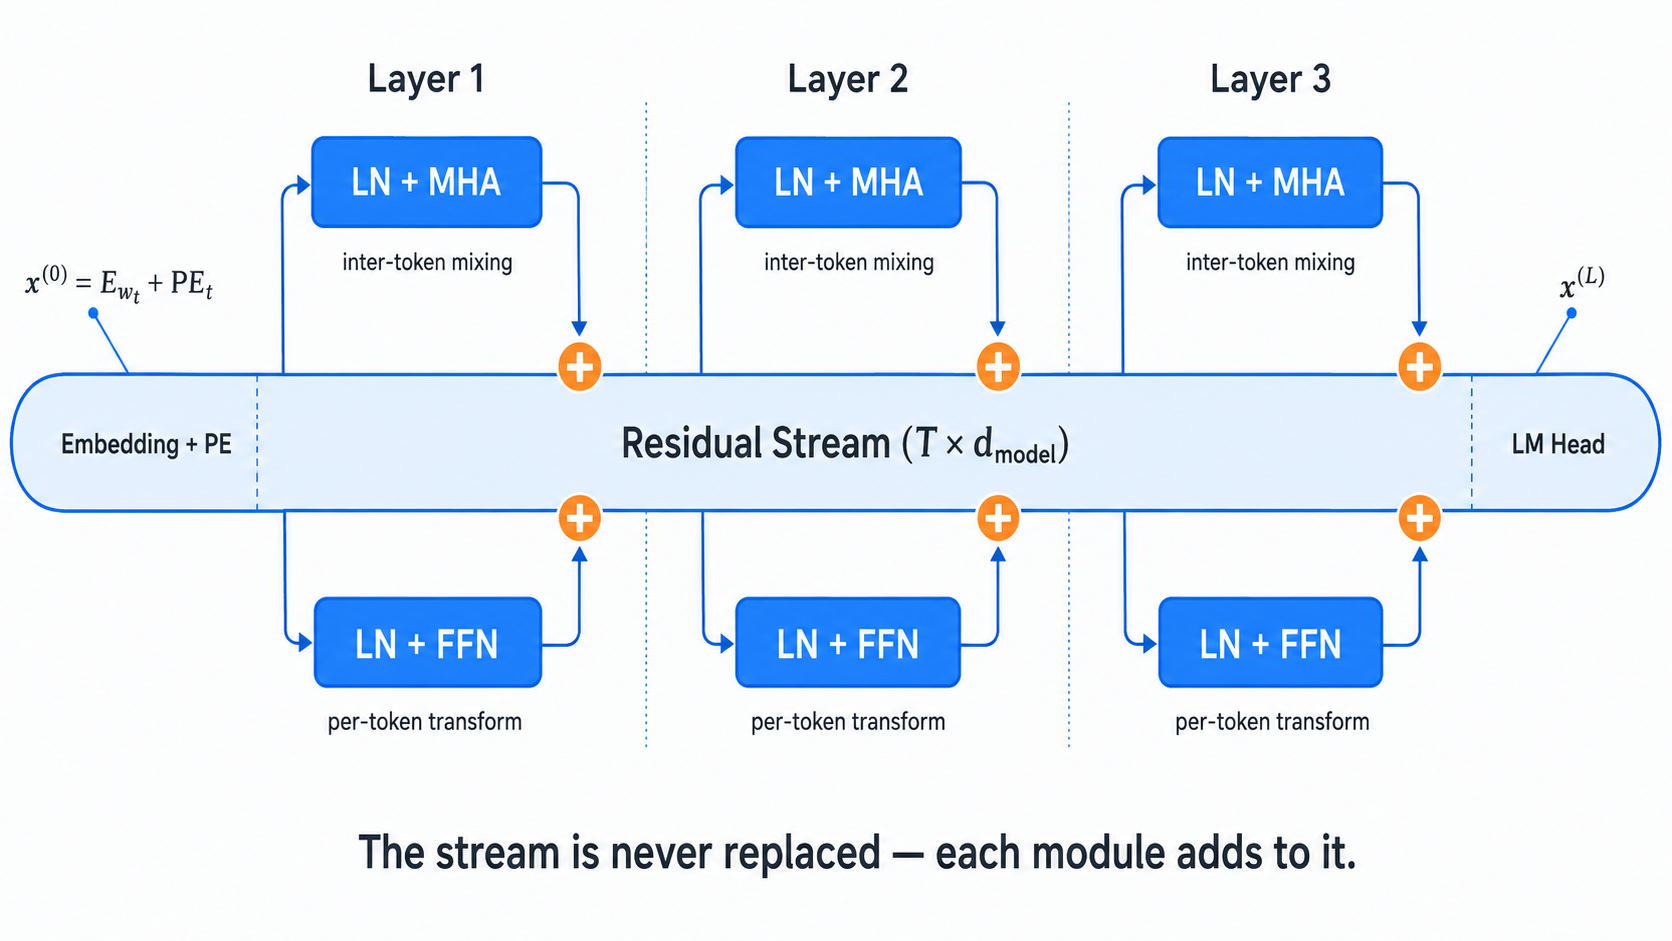
\includegraphics[width=0.75\textwidth]{figures/ch03/residual_stream.png}
  \caption{The residual stream as information highway. The stream (wide horizontal band) flows from embedding to output head. At each layer, attention and FFN modules read from the stream and write additive updates back---the stream itself is never replaced, only enriched. This is the depth analogue of the LSTM cell state (Figure~\ref{fig:lstm-cell}): an additive identity path that enables gradient flow across 100+ layers.}
  \label{fig:residual-stream}
\end{figure}

This additive structure has three consequences that explain why Transformers can be stacked so deep:

\begin{enumerate}[nosep]
  \item \textbf{Gradient highway.} The residual connection creates a direct path from the loss back to any layer. This is the same principle as the LSTM cell state (Chapter~\ref{ch:before-transformer}, \S1.4.3): when the additive updates are small, $\partial \mathbf{x}^{(L)} / \partial \mathbf{x}^{(0)} \approx \mathbf{I}$, and gradients flow without vanishing. This is why Transformers can be stacked 100+ layers deep.

  \item \textbf{Modular read-write.} Attention reads from the stream at all positions and writes a summary back. The FFN reads from the stream at a single position and writes a transformed version back. Each sub-layer is a reader-writer operating on shared memory.

  \item \textbf{Information accumulation.} Early layers typically handle local syntactic patterns; later layers handle longer-range semantic relationships. The residual stream accumulates these contributions---the final representation is a sum of the original embedding plus all intermediate updates.
\end{enumerate}

\paragraph{Analogy to LSTM.} In Chapter~\ref{ch:before-transformer}, the LSTM cell state was a ``gradient highway''---when the forget gate was near 1, information passed through time steps almost unaltered. The residual stream is the same idea applied to \emph{depth} instead of time. The LSTM's cell state carries information across sequence positions; the residual stream carries it across layers. Both work for the same reason: an additive identity path that gradients can flow through without vanishing.

\medskip
\noindent\fbox{\parbox{\dimexpr\textwidth-2\fboxsep-2\fboxrule\relax}{\textbf{Pause and verify.} If you removed the residual connections (so each layer's output replaces the stream instead of adding to it), what would happen to gradient flow in a 32-layer model? How would training behave? (Hint: think about the LSTM without a cell state---which is just a vanilla RNN.)}}

\begin{quickrecap}
\textbf{Quick Recap.}
\begin{itemize}[nosep,leftmargin=1.5em]
  \item The residual stream, not attention, is the backbone of a decoder-only Transformer.
  \item Attention and FFN are reader-writer modules that contribute additive updates to the stream.
  \item Residual connections create gradient highways across depth---the same principle as LSTM cell state, now applied across layers instead of time.
\end{itemize}
\textit{One thing is still missing: the model treats all positions identically. Without position information, ``The cat sat on'' and ``on sat cat The'' produce the same residual stream. How do modern GPTs solve this?}
\end{quickrecap}


%----------------------------------------------------------------------
\section{Position in Modern Decoder-Only Models}
\label{sec:position-modern}

Chapter~\ref{ch:attention} introduced sinusoidal positional encoding: fixed frequency patterns added to the input embeddings. GPT-2 took a simpler route---\textbf{learned absolute positional embeddings}: a trainable matrix $\mathbf{PE} \in \mathbb{R}^{T_{\max} \times d_{\text{model}}}$, one learned vector per position. The model sees enough data to figure out what ``position 37'' should look like. Simple, effective---and flawed in two ways:

\begin{enumerate}[nosep]
  \item \textbf{Hard ceiling on length.} Position 1025 has no embedding if you trained with $T_{\max} = 1024$. The model hits a wall.
  \item \textbf{Absolute, not relative.} ``The adjective is two positions before the noun'' matters more than ``the adjective is at position 37.'' But learned absolute PE encodes only the latter. Two identical sentence fragments at different positions get different representations.
\end{enumerate}

\subsection{RoPE: Rotary Position Embedding}

Most modern decoder-only models---LLaMA, Mistral, Qwen, and their descendants---solve both problems with \textbf{Rotary Position Embedding (RoPE)}~\cite{su2021roformer}. The idea is elegant: instead of adding a position vector to the input embedding, RoPE \emph{rotates} the query and key vectors before computing the attention dot product:
\[
  q_t = R_t \, \mathbf{W}^Q \mathbf{x}_t, \qquad k_s = R_s \, \mathbf{W}^K \mathbf{x}_s
\]
where $R_t$ is a block-diagonal rotation matrix that rotates pairs of dimensions by an angle proportional to position $t$.

The key property: after rotation, the dot product between query at position $t$ and key at position $s$ depends only on the content and the \emph{relative distance} $t - s$:
\[
  q_t^\top k_s = (\mathbf{W}^Q \mathbf{x}_t)^\top R_{t-s} \, (\mathbf{W}^K \mathbf{x}_s)
\]

Why does this matter? Three reasons:
\begin{itemize}[nosep]
  \item \textbf{The residual stream stays clean.} Position is injected into the attention computation, not baked into the embeddings. The stream itself carries only content.
  \item \textbf{No hard ceiling.} The rotation formula works for any position---there is no $T_{\max}$ in the encoding. (The model may still struggle with lengths it has never trained on, but the encoding itself does not break.)
  \item \textbf{Relative position falls out naturally.} Nearby tokens produce small angle differences; distant tokens produce large ones. The model perceives distance without explicit distance features.
\end{itemize}

\begin{figure}[t]
  \centering
  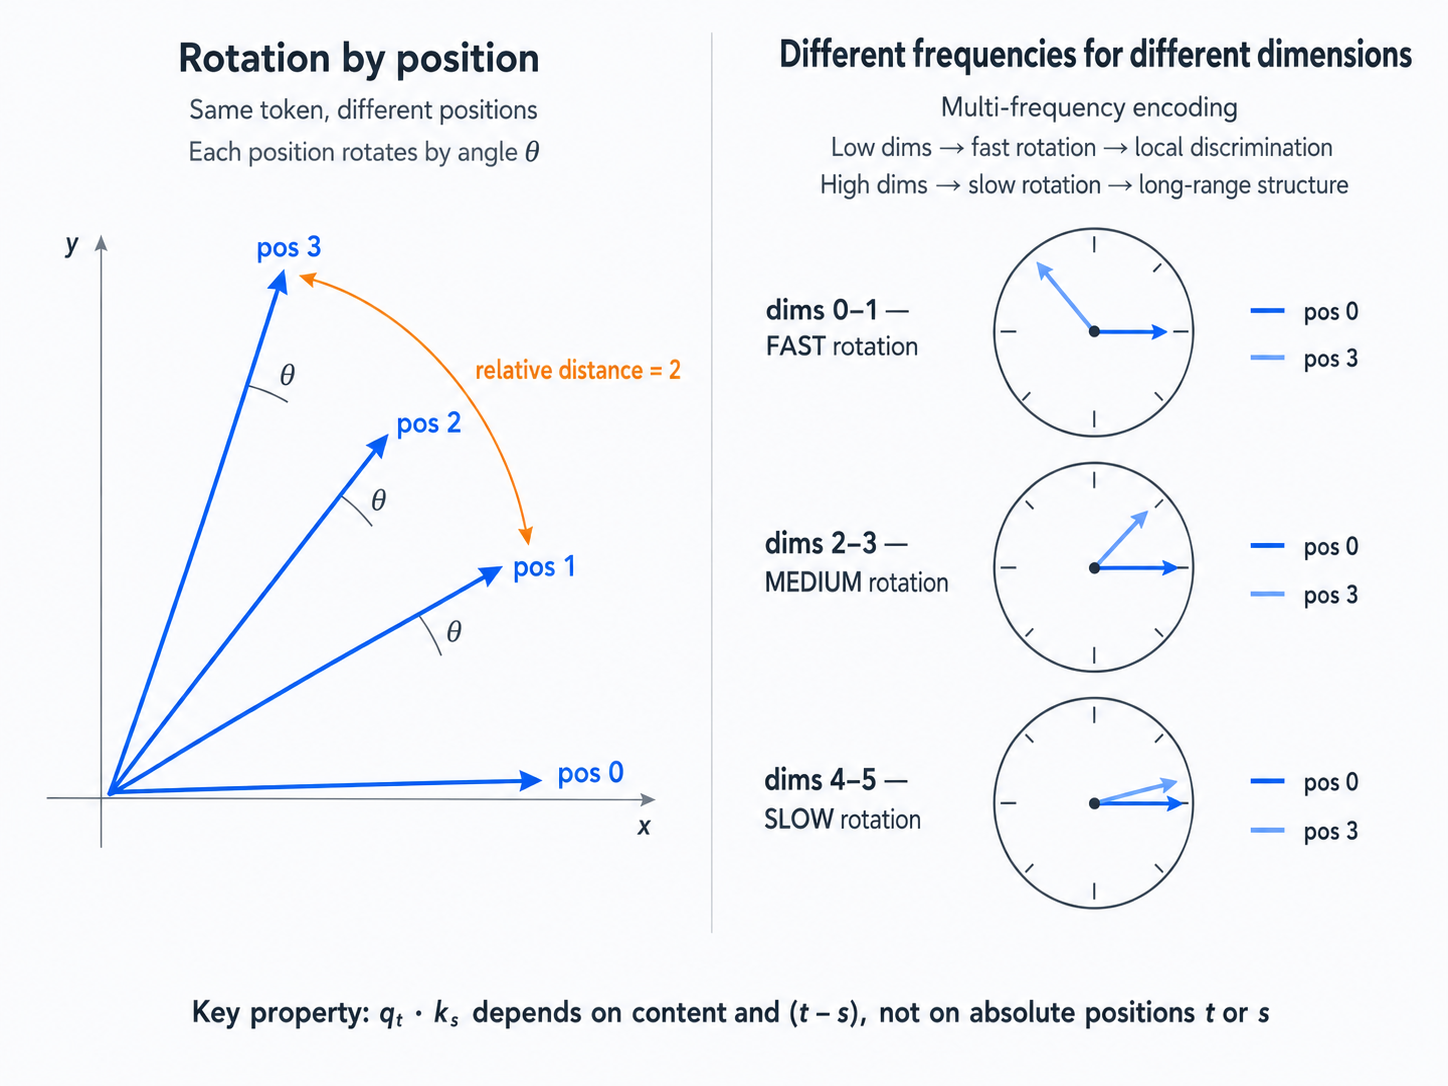
\includegraphics[width=0.85\textwidth]{figures/ch03/rope_rotation.png}
  \caption{Rotary Position Embedding (RoPE) intuition. \textbf{Left:} the same token at different positions is represented by rotating its query/key vectors by an angle proportional to position. The dot product between any two rotated vectors depends only on their angular difference---i.e., relative position $t - s$. \textbf{Right:} different dimension pairs rotate at different frequencies. Low-index pairs rotate fast (distinguishing nearby tokens); high-index pairs rotate slowly (preserving long-range structure).}
  \label{fig:rope-rotation}
\end{figure}

\paragraph{What to remember.} You do not need to memorize rotation matrices. When reading model configs, remember three things: (1)~RoPE is applied to Q and K only---not to V, not to the residual stream; (2)~it encodes relative position through rotation, not addition; (3)~it has become the de facto standard for open-weight LLMs since LLaMA.

\begin{quickrecap}
\textbf{Quick Recap.}
\begin{itemize}[nosep,leftmargin=1.5em]
  \item GPT-2 used learned absolute PE; modern GPTs use RoPE.
  \item RoPE rotates Q and K so that attention scores depend on relative distance, not absolute position.
  \item RoPE is applied inside the attention computation, not added to the embedding.
\end{itemize}
\textit{We have the skeleton of a GPT. Now: what changed between GPT-2 (2019) and LLaMA (2023)? The overall structure stayed the same, but nearly every component inside it was replaced.}
\end{quickrecap}


%----------------------------------------------------------------------
\section{Modern Architecture Choices}
\label{sec:modern-choices}

We now have a working GPT-2--style baseline: learned absolute PE, GELU FFN, standard multi-head attention, pre-norm residual blocks. If you downloaded GPT-2's weights today, this is what you would get---and it would still generate reasonable text.

But between 2019 and 2024, the open-source community ran thousands of ablations at scale and converged on a different recipe. Each change below was driven by a specific engineering pressure: dead neurons, positional ceilings, inference memory, or training instability. None is a theoretical breakthrough; all are battle-tested improvements.

\subsection{Depth vs.\ Width}

Given a fixed parameter budget, should you make the model deeper (more layers $L$) or wider (larger $d_{\text{model}}$)? Parameters scale roughly as $12 L d_{\text{model}}^2$ (see \S\ref{sec:model-scale}), so doubling $d_{\text{model}}$ is much more expensive than doubling $L$.

In practice:
\begin{itemize}[nosep]
  \item \textbf{Wider models} are more stable to train and parallelize better across devices (each layer is independent).
  \item \textbf{Deeper models} can compose more complex functions through layer stacking, but are harder to optimize and more prone to training instabilities.
  \item Modern LLMs (7B--70B) typically use $d_{\text{model}} = 4096$--$8192$ and $L = 32$--$80$, a compromise between depth and width.
\end{itemize}

\subsection[Activation Functions: ReLU to GELU to SwiGLU]{Activation Functions: ReLU $\to$ GELU $\to$ SwiGLU}

The original Transformer used ReLU in the FFN:
\[
  \text{FFN}_{\text{ReLU}}(\mathbf{z}) = \text{ReLU}(\mathbf{z}\mathbf{W}_1 + \mathbf{b}_1)\mathbf{W}_2 + \mathbf{b}_2
\]

\paragraph{The dead neuron problem.} ReLU zeros out every negative input, permanently. In a trained Transformer, a significant fraction of FFN neurons fire for \emph{no} input in the training set---they are ``dead,'' consuming parameters and compute but contributing nothing. Worse, the hard zero boundary creates a discontinuity that can make optimization noisy.

\paragraph{GELU.} GPT-2 and BERT replaced ReLU with GELU (Gaussian Error Linear Unit), which softly attenuates negative inputs instead of hard-killing them. Fewer dead neurons, smoother gradients, marginally better downstream quality.

\begin{figure}[t]
  \centering
  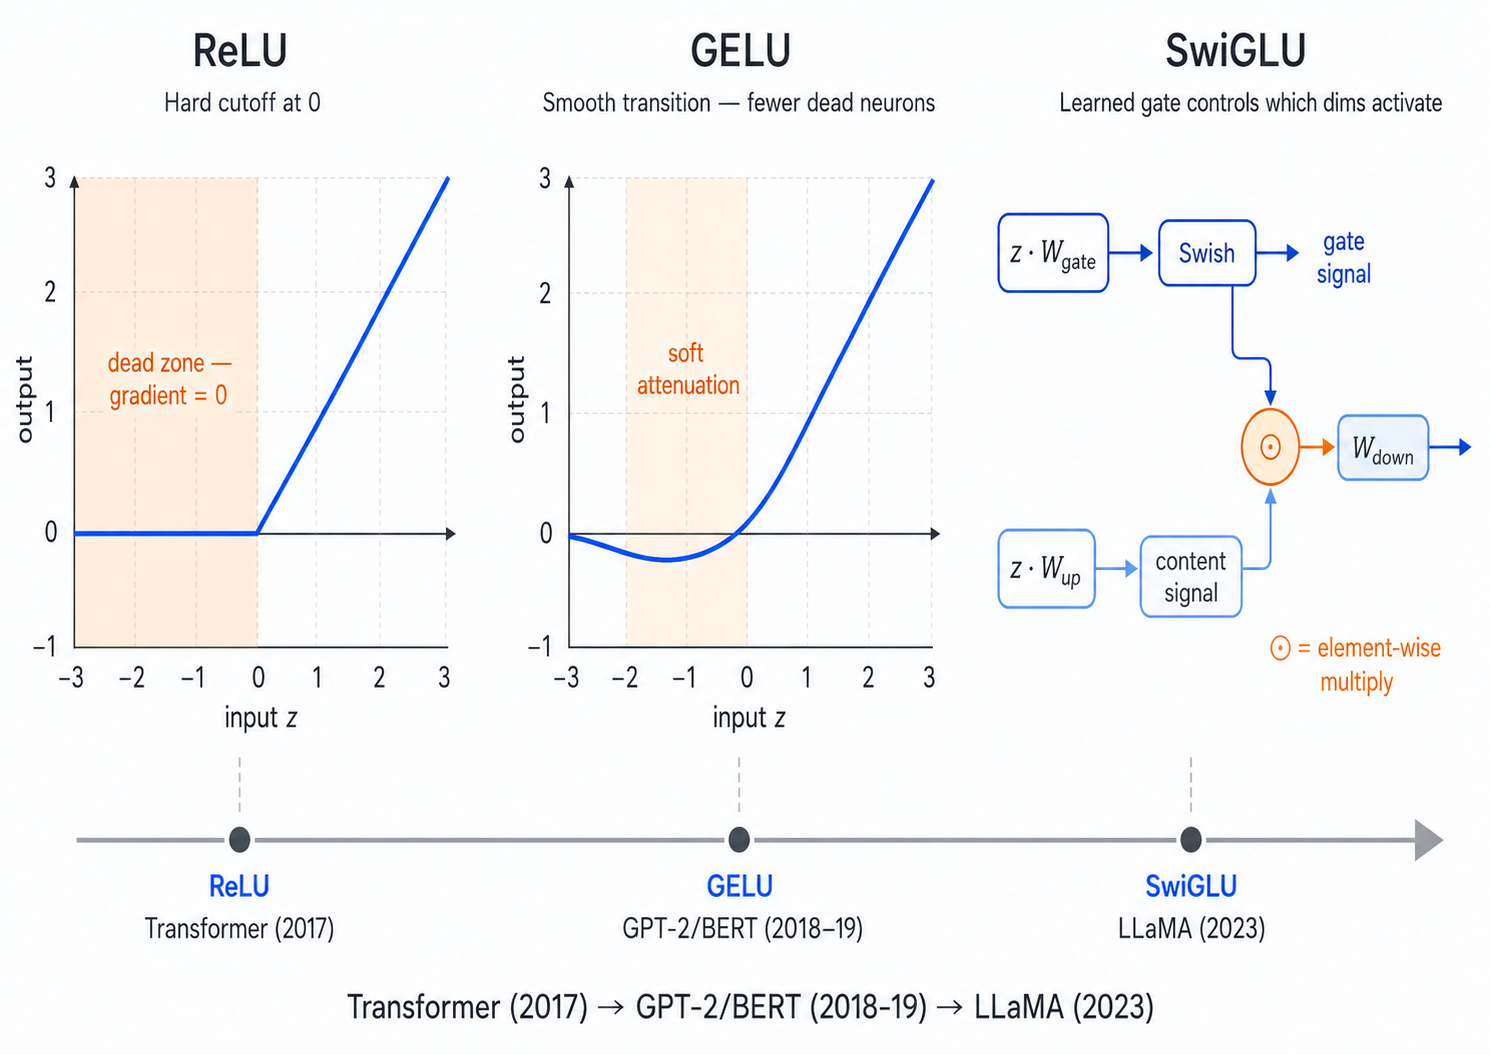
\includegraphics[width=0.9\textwidth]{figures/ch03/activation_functions.png}
  \caption{Activation function evolution in Transformer FFNs. \textbf{Left:} ReLU hard-kills all negative inputs, creating dead neurons (shaded region). \textbf{Center:} GELU softly attenuates negative inputs, reducing dead neurons. \textbf{Right:} SwiGLU adds a learned gate that controls which dimensions activate---the same gating principle as the LSTM, now applied within a single token's FFN computation.}
  \label{fig:activation-functions}
\end{figure}

\paragraph{SwiGLU.} LLaMA and most recent open-weight models go further with SwiGLU~\cite{shazeer2020glu}, which adds a learned \textbf{gating mechanism} to the FFN:
\[
  \text{SwiGLU}(\mathbf{z}) = \big(\text{Swish}(\mathbf{z}\mathbf{W}_{\text{gate}}) \odot (\mathbf{z}\mathbf{W}_{\text{up}})\big) \mathbf{W}_{\text{down}}
\]
One projection ($\mathbf{W}_{\text{gate}}$) decides \emph{which} dimensions to activate; another ($\mathbf{W}_{\text{up}}$) provides the content; a third ($\mathbf{W}_{\text{down}}$) projects back to $d_\text{model}$. If this sounds familiar, it should: it is the same gating principle as the LSTM (Chapter~\ref{ch:before-transformer}). A learned, input-dependent mask controls information flow---except now the ``gate'' operates on hidden dimensions within a single token, not across time.

The cost is a third weight matrix, so to keep the parameter budget constant, the FFN intermediate dimension shrinks from $4 d_{\text{model}}$ to $\frac{8}{3} d_{\text{model}}$. The empirical result: better quality for the same compute.

\subsection{From MHA to GQA}
\label{sec:gqa}

Standard multi-head attention (MHA) has $h$ independent sets of Q, K, and V projections. During autoregressive inference, the K and V vectors for all past tokens must be cached (\S\ref{sec:kv-cache}). This \textbf{KV cache} grows linearly with both sequence length and the number of KV heads, and it often becomes the memory bottleneck during generation.

\textbf{Grouped Query Attention (GQA)} addresses this by sharing K/V heads across groups of query heads. If MHA uses $h = 32$ query heads with $h = 32$ KV heads, GQA might use 32 query heads but only $n_{\text{kv}} = 8$ KV heads. Each group of 4 query heads shares the same K and V projections.

\begin{figure}[t]
  \centering
  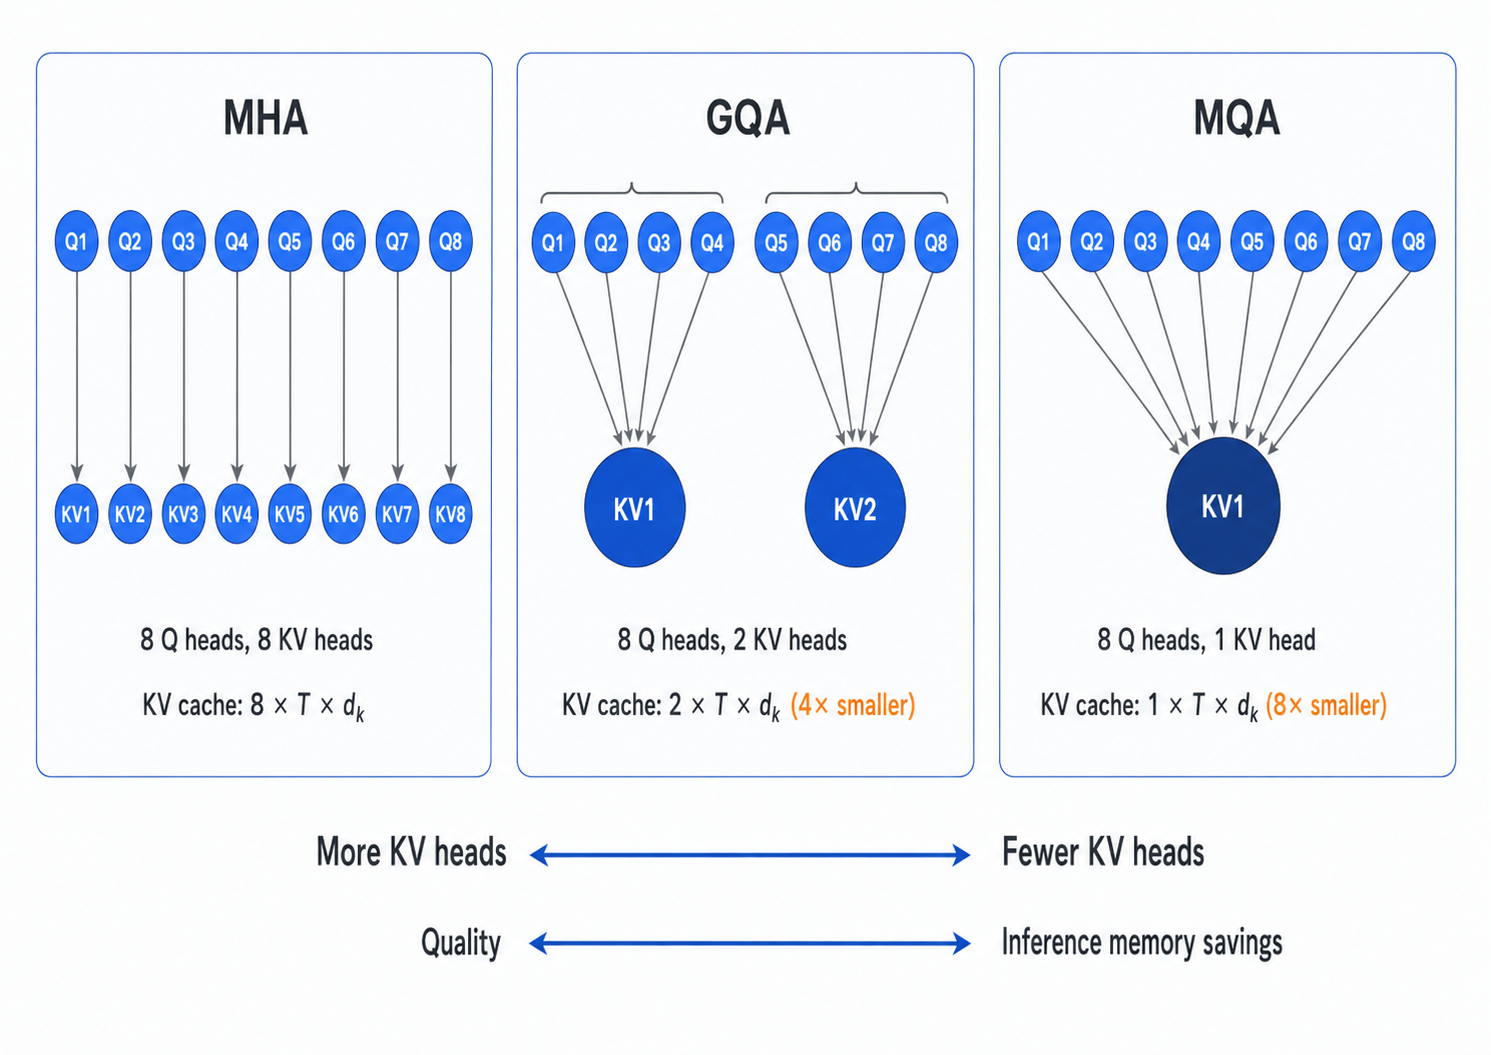
\includegraphics[width=0.9\textwidth]{figures/ch03/mha_vs_gqa.png}
  \caption{Head sharing patterns in multi-head attention variants. \textbf{Left:} Standard MHA---each query head has its own K/V head ($n_\text{kv} = h$). \textbf{Center:} GQA---groups of query heads share K/V heads ($n_\text{kv} < h$), reducing KV cache proportionally. \textbf{Right:} MQA---all query heads share a single K/V head ($n_\text{kv} = 1$), minimizing cache at the cost of potential quality loss.}
  \label{fig:mha-gqa}
\end{figure}

The tradeoff:
\begin{itemize}[nosep]
  \item \textbf{KV cache shrinks by $h / n_{\text{kv}}$.} With $n_{\text{kv}} = 8$ instead of 32, KV cache is $4\times$ smaller. This directly translates to serving more concurrent users or longer contexts on the same hardware.
  \item \textbf{Quality loss is small.} Empirically, going from MHA to GQA with $n_{\text{kv}} = h/4$ causes minimal quality degradation on standard benchmarks.
  \item \textbf{Multi-Query Attention (MQA)} is the extreme case: $n_{\text{kv}} = 1$. All query heads share a single K and V. This minimizes cache but can noticeably hurt quality.
\end{itemize}

\paragraph{Intuition checkpoint.} If a 7B model with 32 KV heads needs about 2.1\,GB of KV cache at context length 4096, how much would GQA with 8 KV heads need? (Answer: roughly $2.1 / 4 \approx 0.5$\,GB---a $4\times$ reduction that directly translates to longer contexts or more concurrent users on the same hardware.)

\subsection{Normalization Placement: Pre-Norm vs.\ Post-Norm}

Chapter~\ref{ch:attention} introduced pre-norm, where LayerNorm is applied \emph{before} each sub-layer. The alternative, \textbf{post-norm}, applies LayerNorm \emph{after} the residual addition:
\begin{align*}
  \text{Pre-norm:} \quad & \mathbf{x}^{(\ell+1)} = \mathbf{x}^{(\ell)} + \text{SubLayer}\!\big(\text{LN}(\mathbf{x}^{(\ell)})\big) \\
  \text{Post-norm:} \quad & \mathbf{x}^{(\ell+1)} = \text{LN}\!\big(\mathbf{x}^{(\ell)} + \text{SubLayer}(\mathbf{x}^{(\ell)})\big)
\end{align*}

Post-norm was used in the original Transformer and some early GPT variants. Pre-norm is now the default because:
\begin{itemize}[nosep]
  \item Pre-norm preserves the gradient highway: the residual identity path is not disrupted by normalization.
  \item Post-norm is more sensitive to initialization and learning rate, requiring careful warmup to avoid early divergence.
  \item Empirically, pre-norm trains more stably at scale, especially beyond 24 layers.
\end{itemize}

Some recent work (e.g., DeepNorm) revisits post-norm with modified residual scaling, but pre-norm remains the practical default.

\begin{quickrecap}
\textbf{Quick Recap.}
\begin{itemize}[nosep,leftmargin=1.5em]
  \item Wider models train more stably; deeper models compose more complex functions. Modern LLMs balance both.
  \item ReLU $\to$ GELU $\to$ SwiGLU: each step reduces dead neurons and adds gated control, at the cost of more parameters.
  \item GQA reduces KV cache memory by sharing K/V heads, with minimal quality loss---critical for inference efficiency.
  \item Pre-norm preserves the gradient highway and trains more stably at depth.
\end{itemize}
\textit{Everything so far describes the model at training time, when all tokens are processed in parallel. Generation is different: the model produces one token at a time, and this changes everything about cost.}
\end{quickrecap}


%----------------------------------------------------------------------
\section{Autoregressive Inference and KV Cache}
\label{sec:kv-cache}

During training, the model processes the entire sequence in parallel: all $T$ tokens pass through all layers simultaneously, and the causal mask prevents each position from seeing the future. Training is a single forward pass per batch---fast, GPU-friendly, and embarrassingly parallel within a sequence.

Inference is a different story. The model generates one token at a time: produce token 1, feed it back, produce token 2, feed it back. Each step depends on the previous one. This sequential constraint---the same one that made RNNs slow---is inherent to autoregressive generation, not to the architecture. But the \emph{cost per step} is something we can optimize.

\subsection{The Naive Approach}

Suppose you have generated 99 tokens and want to produce the 100th. The naive approach recomputes the entire forward pass over all 100 tokens---even though nothing about tokens 1 through 99 has changed since the last step. Generating token 100 repeats all the work of generating token 99, plus a little more.

The waste compounds. Generating 100 tokens naively requires $\sum_{t=1}^{100} O(t^2) \approx O(100^3 / 3)$ attention operations. Most of this is pure redundancy: the K and V vectors for tokens 1 through 99 were already computed on the previous step and did not change.

\subsection{KV Cache: Cache What Does Not Change}

The solution is the \textbf{KV cache}. At each generation step, the model computes K and V only for the \emph{new} token and appends them to a running cache:
\[
  \mathbf{K}_{\text{cache}} \leftarrow \text{concat}(\mathbf{K}_{\text{cache}}, \; \mathbf{k}_t), \qquad
  \mathbf{V}_{\text{cache}} \leftarrow \text{concat}(\mathbf{V}_{\text{cache}}, \; \mathbf{v}_t)
\]
The query for the new token then attends to the full cached history:
\[
  \text{output}_t = \text{Attention}(\mathbf{q}_t, \; \mathbf{K}_{\text{cache}}, \; \mathbf{V}_{\text{cache}})
\]

This reduces per-step cost from $O(t^2)$ to $O(t)$---the new query attends to $t$ cached keys instead of recomputing all pairwise interactions.

\begin{figure}[t]
  \centering
  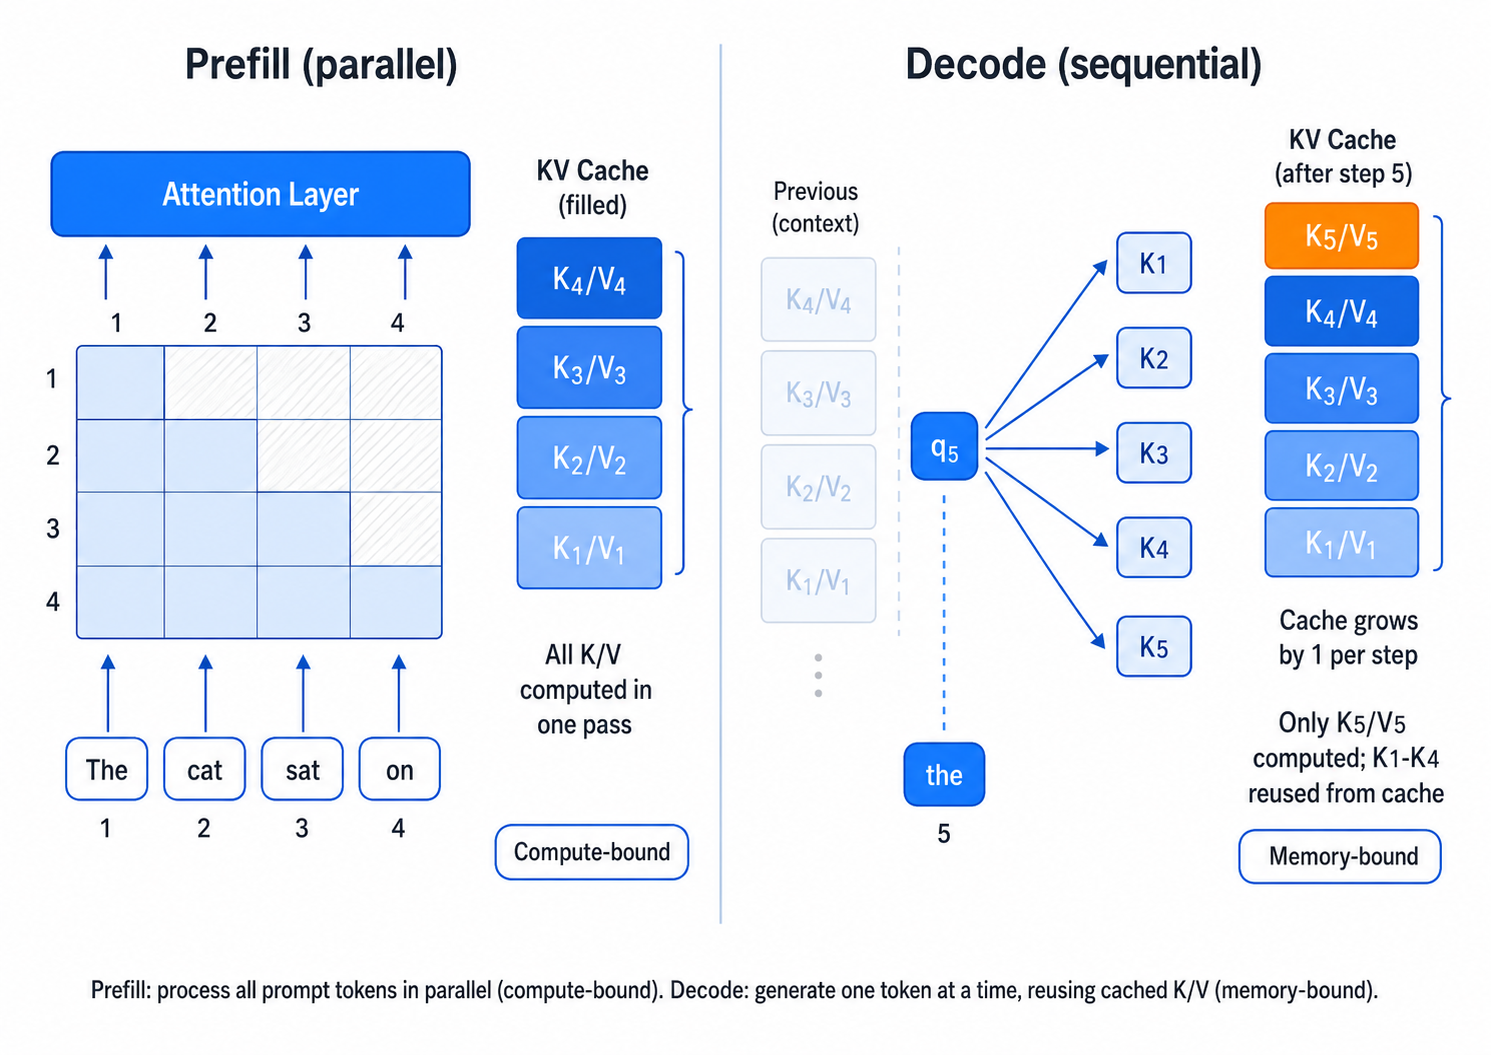
\includegraphics[width=0.85\textwidth]{figures/ch03/kv_cache.png}
  \caption{KV cache during autoregressive generation. \textbf{Left (Prefill):} the full prompt is processed in parallel, filling the cache with K/V vectors for all prompt tokens. \textbf{Right (Decode):} each new token computes only its own Q/K/V, appends K/V to the cache, and attends to the full cached history. The cache (orange) grows by one entry per step; the query (blue) always has size 1.}
  \label{fig:kv-cache}
\end{figure}

\subsection{KV Cache Memory Cost}

The cache stores K and V tensors for every layer and every KV head. For a model with $L$ layers, $n_{\text{kv}}$ KV heads, head dimension $d_k$, and context length $T$, the total cache size is:
\[
  \text{KV cache} = 2 \times L \times n_{\text{kv}} \times T \times d_k \times \text{bytes per element}
\]

\paragraph{Concrete example.} Consider a 7B parameter model (LLaMA-2 7B style):
\begin{itemize}[nosep]
  \item $L = 32$ layers, $n_{\text{kv}} = 32$ heads (MHA), $d_k = 128$, $T = 4096$
  \item Cache per element: 2 bytes (float16)
  \item Total: $2 \times 32 \times 32 \times 4096 \times 128 \times 2 \approx 2.1$\,GB
\end{itemize}

Now with GQA ($n_{\text{kv}} = 8$ instead of 32): $2.1 / 4 \approx 0.5$\,GB. That is the difference between fitting on one GPU and needing two---or equivalently, between serving 4 users and serving 16 on the same hardware. GQA's value is not in training quality; it is in deployment economics.

\medskip
\noindent\fbox{\parbox{\dimexpr\textwidth-2\fboxsep-2\fboxrule\relax}{\textbf{Pause and verify.} The KV cache grows linearly with context length $T$. If you double the context window from 4K to 8K, how does the cache size change? What about the total attention cost of generating $T$ tokens? Are these the same scaling or different?}}

\subsection{Prefill vs.\ Decode}

Autoregressive inference has two phases:

\begin{enumerate}[nosep]
  \item \textbf{Prefill.} The prompt (all input tokens) is processed in parallel, just like training. This fills the KV cache and produces logits for the first generated token. Prefill is compute-bound (lots of matrix multiplications).
  \item \textbf{Decode.} Each subsequent token is generated one at a time. The model computes Q/K/V for one token, appends K/V to the cache, and attends to the full history. Decode is memory-bound (moving the KV cache through memory dominates the cost).
\end{enumerate}

This compute-bound/memory-bound split is why inference optimization for Transformers is fundamentally different from training optimization.

\begin{quickrecap}
\textbf{Quick Recap.}
\begin{itemize}[nosep,leftmargin=1.5em]
  \item Naive generation recomputes everything at each step; KV cache stores past K/V to avoid redundant work.
  \item KV cache size = $2 \times L \times n_\text{kv} \times T \times d_k$ elements. For a 7B model at 4K context: $\sim$2\,GB (MHA) or $\sim$0.5\,GB (GQA).
  \item Prefill is compute-bound (parallel); decode is memory-bound (sequential, one token at a time).
\end{itemize}
\textit{We keep saying ``7B model'' or ``70B model.'' Where do those numbers come from? How many parameters does each component contribute?}
\end{quickrecap}


%----------------------------------------------------------------------
\section{What Makes a Model ``Large''?}
\label{sec:model-scale}

``A 7B model''---but 7 billion \emph{what}? Where do the parameters live? Understanding the parameter budget is essential for choosing between models, estimating GPU requirements, and reading scaling-law papers. A decoder-only Transformer has three main groups:

\paragraph{1. Embedding.} $V \times d_{\text{model}}$ parameters. With weight tying, the output head is free. For $V = 32{,}000$ and $d_{\text{model}} = 4096$: $\sim$131M.

\paragraph{2. Attention.} Each layer has Q, K, V, and output projections. For standard MHA: $4 \times d_{\text{model}}^2$ per layer. With $L$ layers: $4L d_{\text{model}}^2$. For GQA with $n_{\text{kv}}$ KV heads and $h$ query heads ($d_k = d_{\text{model}} / h$): the K/V projections shrink to $2 \times n_{\text{kv}} \times d_k \times d_{\text{model}}$.

\paragraph{3. FFN.} For SwiGLU with three projections of size $d_{\text{model}} \times d_{\text{ff}}$: $3 d_{\text{model}} \times d_{\text{ff}}$ per layer. With $d_{\text{ff}} = \frac{8}{3} d_{\text{model}}$: $8 d_{\text{model}}^2$ per layer, totaling $8L d_{\text{model}}^2$.

\paragraph{Rough total.} Ignoring biases and normalization parameters (which are negligible), the total is approximately:
\[
  \text{Params} \approx V \cdot d_{\text{model}} + L \cdot (4 d_{\text{model}}^2 + 8 d_{\text{model}}^2) = V \cdot d_{\text{model}} + 12 L \, d_{\text{model}}^2
\]
For large models, the $12 L d_{\text{model}}^2$ term dominates. This is why model size scales primarily with depth times width squared.

\paragraph{Scale comparison.}

\begin{center}
\begin{tabular}{lrrrr}
\toprule
\textbf{Model} & \textbf{Params} & $L$ & $d_{\text{model}}$ & $h$ \\
\midrule
GPT-2 Small   &   117M &  12 &   768 &  12 \\
GPT-2 XL      &  1.5B  &  48 &  1600 &  25 \\
LLaMA-2 7B    &  6.7B  &  32 &  4096 &  32 \\
LLaMA-2 70B   & 70B    &  80 &  8192 &  64 \\
\bottomrule
\end{tabular}
\end{center}

\noindent From GPT-2 Small to LLaMA-2 70B, depth grew $\sim$7$\times$ and width grew $\sim$11$\times$---but parameters grew $\sim$600$\times$. The asymmetry comes from the $d_\text{model}^2$ term: doubling width quadruples the per-layer parameter count. This is why scaling discussions focus on width as much as depth.

\paragraph{Looking ahead.} More parameters generally mean lower loss---but the relationship is not linear, and the returns diminish. How much data does a 70B model need? How much compute? Is it better to train a smaller model on more data, or a larger model on less? These questions have quantitative answers, and they go by the name of \emph{scaling laws}. We cover them in Part~II.

\begin{quickrecap}
\textbf{Quick Recap.}
\begin{itemize}[nosep,leftmargin=1.5em]
  \item Total parameters $\approx V \cdot d_\text{model} + 12 L \, d_\text{model}^2$. FFN typically accounts for $\sim$2/3 of the per-layer parameters.
  \item From GPT-2 to LLaMA-2 70B: $\sim$600$\times$ more parameters, driven primarily by width.
  \item More parameters $\to$ lower loss, but not linearly. Scaling laws (Part~II) formalize this relationship.
\end{itemize}
\end{quickrecap}


%----------------------------------------------------------------------
\section{Failure Modes and Common Misconceptions}

Before moving to the summary, it is worth confronting five misconceptions that commonly arise after a first reading of this material. These are not pedantic distinctions---each one, if left uncorrected, will cause confusion in later chapters on scaling, inference optimization, and architecture search.

\begin{itemize}
  \item \textbf{``Decoder-only means the model can only generate.''} This confuses architecture with capability. When GPT answers a question, the question is the prefix---the model ``understands'' it by using it as context for next-token prediction. The distinction between understanding and generation is about training objective and data format, not about whether the architecture has an encoder.

  \item \textbf{``KV cache eliminates the quadratic cost of attention.''} KV cache reduces per-step cost from $O(t^2)$ to $O(t)$, but the \emph{total} cost of generating $T$ tokens is still $O(T^2)$: step 1 attends to 1 key, step 2 attends to 2, \ldots, step $T$ attends to $T$. The sum is $O(T^2/2)$. What KV cache eliminates is \emph{redundant recomputation}, not the fundamental quadratic scaling.

  \item \textbf{``Weight tying always helps.''} Weight tying is beneficial when the vocabulary is large relative to $d_{\text{model}}$, because it removes a huge parameter block and regularizes the model. But for very large models with small vocabularies, the embedding and output head may benefit from learning different representations. Some recent large models (e.g., PaLM) untie the weights.

  \item \textbf{``Deeper is always better.''} Beyond a certain depth, adding layers gives diminishing returns or actively hurts training stability. The relationship between depth, width, and quality is task-dependent and budget-dependent. Scaling laws, not intuition, should guide this decision.

  \item \textbf{``GQA is just a quality-speed tradeoff.''} GQA's primary benefit is \emph{memory} savings (smaller KV cache), not speed per se. During prefill, GQA and MHA have similar compute costs. The savings appear during decode, where KV cache size determines batch capacity and maximum context length.
\end{itemize}


\section{Trick Table}

\noindent
\begin{tabularx}{\textwidth}{@{}>{\raggedright\arraybackslash}p{2.8cm}
                              >{\raggedright\arraybackslash}p{2.8cm}
                              >{\raggedright\arraybackslash}p{3.2cm}
                              X@{}}
\toprule
\textbf{Trick} & \textbf{When to use} & \textbf{Expected effect} & \textbf{Failure signal} \\
\midrule
Weight tying &
  Models with large vocab; default for most LLMs &
  Saves $V \times d$ parameters; regularizes embedding space &
  Untied heads may help if vocab is small relative to $d$ \\[4pt]
RoPE &
  Default for modern decoder-only LLMs &
  Relative position encoding; better length generalization &
  Weak performance past the trained context window \\[4pt]
SwiGLU FFN &
  Modern LLMs (LLaMA, Mistral, etc.) &
  Gated activation reduces dead neurons; smoother loss landscape &
  Requires reducing $d_\text{ff}$ to compensate for extra parameters \\[4pt]
GQA ($n_\text{kv} < h$) &
  Inference-heavy deployment &
  KV cache shrinks by $h / n_\text{kv}$; minimal quality loss &
  Too few KV heads ($n_\text{kv} = 1$) may hurt quality on complex tasks \\[4pt]
Pre-norm &
  Any Transformer deeper than $\sim$12 layers &
  More stable training; avoids early divergence &
  Slightly different final-layer dynamics than post-norm \\
\bottomrule
\end{tabularx}


\begin{takeaways}
\begin{itemize}[leftmargin=1.2em, itemsep=4pt]
  \item Decoder-only Transformers became the LLM default because next-token prediction is a universal objective that requires no paired data and concentrates the model's capacity in a single causal language-modeling stack.
  \item The \textbf{residual stream} is the model's backbone: a persistent $T \times d_\text{model}$ representation that attention and FFN modules read from and write to. It is the gradient highway that enables deep stacking.
  \item \textbf{Weight tying} between embedding and output projection saves hundreds of millions of parameters and enforces consistency between input and output spaces.
  \item Modern GPTs replace ReLU with \textbf{SwiGLU} (gated FFN), learned PE with \textbf{RoPE} (relative position through rotation), and MHA with \textbf{GQA} (shared KV heads for inference efficiency).
  \item \textbf{KV cache} eliminates redundant computation during autoregressive generation, but the cache itself becomes a memory bottleneck---which is why GQA matters.
  \item Total parameters $\approx 12 L d_\text{model}^2$; FFN dominates. Scaling is primarily driven by width ($d_\text{model}^2$), not depth.
  \item The architecture decisions in this chapter were validated empirically over years of scaling experiments. They are engineering choices, not theoretical necessities---and they may evolve.
\end{itemize}
\end{takeaways}


\section{Summary}

\paragraph{What this chapter built.} Chapter~\ref{ch:attention} gave us the components; this chapter assembled them into a machine. The result is a decoder-only Transformer that reads a prefix, passes it through a residual stream enriched by attention and FFN modules at each layer, and predicts the next token from the top of the stack. The entire model trains on one objective---cross-entropy on shifted labels---using every token in every document as supervision.

\paragraph{The key conceptual shift.} A decoder-only Transformer is not a ``stack of attention layers.'' It is a \textbf{residual stream}---a persistent $T \times d_\text{model}$ representation---with attention and FFN modules that read from and write to it. This is the gradient highway that enables 100+ layers of depth, and it is the direct descendant of the LSTM cell state from Chapter~\ref{ch:before-transformer}.

\paragraph{From GPT-2 to LLaMA.} We traced a specific evolutionary path: learned absolute PE gave way to RoPE (relative position through rotation); GELU gave way to SwiGLU (gated FFN with fewer dead neurons); MHA gave way to GQA (shared KV heads for inference memory). Each replacement was driven by a concrete engineering pressure, and each was validated by thousands of ablations at scale. The architecture diagram barely changed---but the components inside it were systematically upgraded.

\paragraph{What comes next.} This chapter covered what a GPT \emph{is}. It did not cover how to \emph{train} one---learning rate schedules, initialization, mixed-precision arithmetic, distributed strategies, and the scaling laws that dictate how much data and compute a given model size requires. Those are the subjects of Part~II. Before that, Chapter~\ref{ch:bert} examines the other major branch of Transformer models: encoder-only architectures like BERT, which use the same mechanism but make fundamentally different choices---bidirectional attention and masked language modeling instead of causal next-token prediction.

\medskip
\noindent\textit{Self-check: revisit the Learning Objectives. Can you trace a full GPT forward pass? Can you explain the residual stream, weight tying, RoPE, SwiGLU, GQA, and KV cache? Can you estimate the parameter count of a Transformer from its config? If any point is unclear, re-read the corresponding section before continuing.}


\section*{Key Equations at a Glance}

\begin{center}
\renewcommand{\arraystretch}{1.6}
\begin{tabularx}{\textwidth}{@{}lX@{}}
\toprule
Component & Equation \\
\midrule
Input embedding & $\mathbf{x}_t^{(0)} = \mathbf{E}_{w_t} + \mathbf{PE}_t$ \\[4pt]
Pre-norm block (step 1) & $\mathbf{z}^{(\ell)} = \mathbf{x}^{(\ell)} + \text{MHA}\!\big(\text{LN}(\mathbf{x}^{(\ell)})\big)$ \\[4pt]
Pre-norm block (step 2) & $\mathbf{x}^{(\ell+1)} = \mathbf{z}^{(\ell)} + \text{FFN}\!\big(\text{LN}(\mathbf{z}^{(\ell)})\big)$ \\[4pt]
LM head (tied) & $\text{logits}_t = \mathbf{E}^\top \, \text{LN}(\mathbf{x}_t^{(L)})$ \\[4pt]
Shifted CE loss & $\mathcal{L} = -\frac{1}{T-1}\sum_{t=1}^{T-1} \log P_\theta(w_{t+1} \mid w_{\leq t})$ \\[4pt]
RoPE & $q_t^\top k_s$ depends on content and relative distance $t - s$ \\[4pt]
SwiGLU & $\text{SwiGLU}(\mathbf{z}) = (\text{Swish}(\mathbf{z}\mathbf{W}_\text{gate}) \odot \mathbf{z}\mathbf{W}_\text{up})\,\mathbf{W}_\text{down}$ \\[4pt]
KV cache size & $2 \times L \times n_\text{kv} \times T \times d_k \times \text{bytes}$ \\[4pt]
Param estimate & $\text{Params} \approx V \cdot d_\text{model} + 12 L \, d_\text{model}^2$ \\
\bottomrule
\end{tabularx}
\end{center}


\section*{Lab 3: What Holds a GPT Together}

\subsection*{Goal}

Lab~2 started with a working Transformer and removed ingredients one at a time. Lab~3 inverts the method: you start with a \emph{barely functional} tiny decoder-only GPT and progressively add the structural features that make it correct, trainable, and fast. The central finding: without the residual stream a deep decoder-only model trains poorly or unstably; with it, even a 4-layer model can produce recognizable text.

\subsection*{Expected Time}

Core (Experiments~0--3 + Cross-lab comparison): 5--7 hours. Optional extensions: 1--2 hours each.

\subsection*{Setup}

See \texttt{labs/ch03/README.md} for the full specification. We provide a runnable scaffold for a configurable mini GPT (2--8 layers, \texttt{d\_model}=128--256, 4 heads). The scaffold includes the model, data loading (Tiny Shakespeare, the same dataset as Lab~1), a training loop, generation utilities, and profiling scripts.

\noindent This is an \textbf{experiment-first lab}: your time goes into running controlled comparisons, interpreting results, and writing the report---not debugging data pipelines. You should still read the model code carefully, because each experiment is designed to test one structural choice in that code.

\subsection*{Verify}

Before running experiments, confirm these sanity checks on the baseline:

\begin{enumerate}[nosep]
    \item \textbf{Logits shape.} Output should be \texttt{[B, T, V]} where \texttt{V} matches vocabulary size.
    \item \textbf{Causal mask.} Modify a future token; output at earlier positions must not change.
    \item \textbf{Weight tying.} If enabled, \texttt{model.embedding.weight} and \texttt{model.lm\_head.weight} should point to the same tensor (check with \texttt{is}).
    \item \textbf{KV cache consistency.} In \texttt{model.eval()} mode, full-sequence and incremental cached forward passes should produce identical logits when position offsets are handled correctly.
\end{enumerate}

\subsection*{Experiment 0: Shifted-Label Bug Hunt}

\textbf{Corresponds to:} \S3.2 (shifted cross-entropy loss).

\textbf{Goal:} Diagnose a deliberate off-by-one bug in the loss computation.

The experiment script trains one model with a deliberately buggy no-shift loss and another with the correct shifted cross-entropy loss. The buggy model ``predicts'' the token it already sees instead of the next token. This is analogous to Lab~2's missing causal mask: the training loss looks good, but the model learns nothing useful.

\begin{enumerate}[nosep]
    \item Train with the buggy no-shift loss for 500 steps. Note the suspiciously low loss.
    \item Generate 200 characters. Observe: the output is incoherent despite the low loss.
    \item Diagnose the problem: the model is copying, not predicting.
    \item Compare against \texttt{shifted\_ce\_loss}: each logit at position $t$ predicts the token at position $t+1$.
    \item Retrain with the correct loss. The loss will be higher, but generation will be more coherent.
\end{enumerate}

\textbf{Report:} Side-by-side comparison of buggy vs.\ fixed loss curves and generated samples.

\subsection*{Experiment 1: Residual Stream and Normalization (Centerpiece)}

\textbf{Corresponds to:} \S3.3 (residual stream), \S3.8 (failure modes).

\textbf{Goal:} Demonstrate that the residual stream is the backbone of a trainable deep Transformer, and that normalization placement matters.

Train three 8-layer models on Tiny Shakespeare, identical except for architecture:

\begin{enumerate}[nosep]
    \item \textbf{No residual connections.} Each block is $\mathbf{Y} = \text{FFN}(\text{MHA}(\mathbf{X}))$---no skip.
    \item \textbf{Post-norm with residual.} Original Vaswani placement: normalize \emph{after} the residual addition.
    \item \textbf{Pre-norm with residual.} Modern GPT placement: normalize \emph{before} each sub-layer.
\end{enumerate}

\noindent Record at every step: training loss and gradient norm (on all parameters).

\textbf{What to look for:}
\begin{itemize}[nosep]
    \item No-residual model: does the loss decrease at all? Do gradient norms explode, vanish, or fluctuate wildly? Look for degradation, instability, or much slower learning rather than assuming every run will collapse.
    \item Post-norm model: does it train, but with occasional loss spikes? Are gradient norms less stable than pre-norm?
    \item Pre-norm model: smooth training, stable gradient norms. This is the GPT default for a reason.
\end{itemize}

\textbf{Key deliverable:} One figure with gradient norm vs.\ training step, three curves overlaid. This is the centerpiece figure of Lab~3---it should make the residual stream's role as a gradient highway immediately visible.

\textbf{Connection to Lab~1:} Compare this figure with your Lab~1 gradient norm plot (vanilla RNN vs.\ LSTM). The structural parallel is direct: LSTM cell state stabilizes gradient flow through time; the residual stream stabilizes gradient flow through depth. Note where the analogy holds and where it breaks.

\subsection*{Experiment 2: Positional Encoding}

\textbf{Corresponds to:} \S3.4 (position in decoder-only models).

\textbf{Goal:} Verify that without explicit positional information, a decoder-only Transformer has an incomplete order signal---and compare encoding strategies.

Train three models (4 layers, pre-norm, with residual):

\begin{enumerate}[nosep]
    \item \textbf{No positional encoding.}
    \item \textbf{Learned absolute PE} (GPT-2 style).
    \item \textbf{RoPE} (LLaMA style), if your scaffold supports it.
\end{enumerate}

\textbf{What to look for:}
\begin{itemize}[nosep]
    \item No PE: validation loss should be noticeably worse, and generated text may show weaker ordering. The causal mask still tells each position which tokens are visible, but the model cannot directly distinguish relative positions within the visible prefix.
    \item Learned PE vs.\ RoPE: in a short training run on a small model, the difference may be subtle. Do \emph{not} force a conclusion that ``RoPE is better.'' Instead, note that RoPE's advantage---relative position generalization---primarily manifests at longer contexts than this lab uses.
\end{itemize}

\textbf{Report:} Validation loss table for all three configurations. 200-character generated samples from each. One sentence on whether the no-PE model's output shows weaker ordering.

\subsection*{Experiment 3: KV Cache Profiling}

\textbf{Corresponds to:} \S3.6 (autoregressive inference and KV cache).

\textbf{Goal:} See with your own eyes that KV cache transforms the cost structure of autoregressive generation.

Using the pre-norm baseline (Experiment~1, configuration~3):

\begin{enumerate}[nosep]
    \item Generate 512 tokens \emph{without} KV cache (recompute all attention from scratch at every step). Record the wall-clock time for each generated token.
    \item Generate 512 tokens \emph{with} KV cache. Record per-token times.
    \item Plot: \textbf{milliseconds per token vs.\ token position}, two curves.
\end{enumerate}

\textbf{What to look for:}
\begin{itemize}[nosep]
    \item Without cache: time per token should increase roughly linearly with position (each step recomputes attention over a growing context).
    \item With cache: time per token should be approximately constant (each step only computes attention for the new token against cached keys/values).
    \item The total generation time for 512 tokens should be dramatically different.
\end{itemize}

\textbf{Optional:} Estimate KV cache memory at context lengths 256, 512, 1024, and 2048 using the formula from \S3.6. Compare with measured GPU memory via \texttt{torch.cuda.memory\_allocated()}.

\subsection*{Cross-Lab Comparison: LSTM vs.\ Transformer}

\textbf{Corresponds to:} Ch.~1 $\to$ Ch.~3 narrative arc.

\textbf{Goal:} Close the loop between Lab~1 and Lab~3 by comparing architectures on the same task.

Use the pre-norm Transformer from Experiment~1 and the LSTM from Lab~1, both trained on Tiny Shakespeare with approximately matched parameter counts:

\begin{center}
\begin{tabular}{lll}
\toprule
& LSTM & Transformer \\
\midrule
Layers & 2 & 4 \\
Hidden / $d_\text{model}$ & 512 & 256 \\
Approx.\ params & $\sim$5M & $\sim$5M \\
\bottomrule
\end{tabular}
\end{center}

Compare: validation loss, training throughput (tokens/sec), and 200-character generated samples. The Transformer may or may not win on this tiny task---that is fine. The point is to observe \emph{qualitative} differences in training dynamics and generation style.

\subsection*{Optional Extensions}

\begin{enumerate}
    \item \tierstretch{} \textbf{Learned residual gate.} Replace the additive residual ($\mathbf{x} + f(\mathbf{x})$) with a learned gate: $\alpha \cdot \mathbf{x} + (1 - \alpha) \cdot f(\mathbf{x})$, where $\alpha$ is a scalar parameter initialized to 0.9. After training, inspect $\alpha$---does it stay close to 1.0? What does this tell you about how much the model relies on the residual stream vs.\ the sub-layer output?
    \item \tierstretch{} \textbf{Depth scaling.} Train pre-norm models with 2, 4, 8, and 16 layers (adjusting width to keep total parameters roughly constant). Plot validation loss vs.\ depth. Is there a sweet spot?
    \item \tierstretch{} \textbf{GQA profiling.} If your scaffold supports grouped query attention, compare KV cache memory usage between MHA (all heads have independent K/V) and GQA (shared K/V heads). Measure the memory difference at context length 2048.
\end{enumerate}

\subsection*{Deliverables}

\begin{itemize}[nosep]
    \item Runnable code for all experiments, with clear instructions.
    \item Verification notes: one sentence per sanity check.
    \item Figures: buggy vs.\ fixed loss curves (Exp~0), gradient norm plot with three curves (Exp~1, \textbf{centerpiece}), ms/token vs.\ position (Exp~3).
    \item Tables: PE comparison (Exp~2), LSTM vs.\ Transformer (Cross-lab).
    \item A 600--800 word experiment report (see below).
\end{itemize}

\subsection*{Evaluation Rubric}

\begin{center}
\begin{tabular}{lp{0.7\textwidth}}
\toprule
Weight & Criteria \\
\midrule
10\% & Setup: model trains correctly; all four sanity checks pass. \\
15\% & Experiment 0: off-by-one bug correctly identified and diagnosed using the buggy-vs.\ fixed comparison. \\
30\% & Experiment 1 (\textbf{centerpiece}): gradient norm plot clearly shows three regimes. Diagnosis connects residual stream to gradient highway. Explicit comparison with Lab~1's RNN vs.\ LSTM gradient plot. \\
15\% & Experiments 2--3: PE comparison and KV cache profiling are quantitative and honestly interpreted. \\
20\% & Experiment report: causal reasoning connecting results to Ch.~3 theory. Includes cross-lab comparison. \\
10\% & Reproducibility: code, configs, and seeds documented. \\
\bottomrule
\end{tabular}
\end{center}


\section*{Experiment Report}

Write a 600--800 word report structured around one question: \emph{what makes a decoder-only Transformer correct, trainable, and fast?}

\begin{description}[style=nextline, leftmargin=1.5em]
    \item[Question.] What makes a decoder-only Transformer correct, trainable, and fast---and which properties come from the architecture vs.\ the training objective?
    \item[Setup.] Model, data, hyperparameters. Note what was held constant across experiments.
    \item[Interventions.] For each experiment, name what was changed and why.
    \item[Results.] The headline numbers and figures. The Exp~1 gradient norm plot is the centerpiece---spend the most space here.
    \item[Diagnosis.] Connect each result to the corresponding Ch.~3 claim. The residual-stream--gradient-highway parallel with Lab~1's LSTM cell state is the linchpin.
    \item[Next step.] If you had one more day, what would you investigate?
\end{description}

\noindent\textit{A strong report includes a direct comparison between the Lab~1 gradient norm plot (RNN vs.\ LSTM) and the Lab~3 gradient norm plot (no-residual vs.\ pre-norm). The structural parallel---cell state as temporal gradient highway, residual stream as depth gradient highway---should be supported by your measurements, not just asserted.}


\section*{Key Readings}

\nocite{vaswani2017attention,radford2018improving}

\begin{description}[style=nextline, leftmargin=1.5em]
  \item[Radford et al.\ (2018). \normalfont\textit{Improving Language Understanding by Generative Pre-Training.} OpenAI.]
  Read for: GPT-1---the first decoder-only Transformer language model. Focus on the architecture decisions (decoder-only, learned PE, pre-norm) and how a single pretrained model was fine-tuned for diverse tasks.

  \item[Radford et al.\ (2019). \normalfont\textit{Language Models are Unsupervised Multitask Learners.} OpenAI.]
  Read for: GPT-2---same architecture as GPT-1 but $10\times$ larger ($1.5$B params) and trained on a larger, more diverse dataset. The key insight is zero-shot transfer: a language model can perform tasks it was never explicitly trained for.

  \item[Touvron et al.\ (2023). \normalfont\textit{LLaMA: Open and Efficient Foundation Language Models.} Meta.]
  Read for: the modern decoder-only recipe that became the open-weight standard. Focus on the architecture choices: RoPE, SwiGLU, and pre-norm/RMSNorm. GQA becomes important in later open-weight recipes and larger inference-oriented variants. This paper crystallizes the ``best practices'' of 2023.

  \item[Su et al.\ (2021). \normalfont\textit{RoFormer: Enhanced Transformer with Rotary Position Embedding.} arXiv.]
  Read for: the original RoPE paper. The mathematical derivation is dense, but Sections 3.1--3.3 give sufficient intuition for why rotation encodes relative position.

  \item[Shazeer (2020). \normalfont\textit{GLU Variants Improve Transformer.} arXiv.]
  Read for: the systematic comparison of gated linear units (including SwiGLU) in Transformer FFNs. Short paper with clear ablations.
\end{description}

\bigskip
\noindent\textbf{What's next.}\quad This chapter covered the decoder-only architecture. Chapter~\ref{ch:bert} examines the other major branch of Transformer models: encoder-only architectures like BERT, which use bidirectional attention and masked language modeling to learn general-purpose text representations.
